\documentclass[10pt]{beamer}

\makeatother

\usepackage[utf8]{inputenc}
\usepackage{color}
\usecolortheme{beaver}

\usenavigationsymbolstemplate{}
\setbeamertemplate{footline}[frame number]
\graphicspath{{images/}} 

\usepackage{appendixnumberbeamer}
\usepackage{booktabs}
\usepackage[scale=2]{ccicons}
\usepackage{pgfplots}
\usepgfplotslibrary{dateplot}
%\pgfplotsset{compat=1.15}
\usepackage{tabularx}
\usepackage{xspace}
\usepackage{xcolor}
\definecolor{cmarkcolor}{RGB}{116, 209, 105}
\definecolor{xmarkcolor}{RGB}{230, 25, 25}
\newcommand{\cmark}{\color{cmarkcolor}\ding{51}}%
\newcommand{\xmark}{\color{xmarkcolor}\ding{55}}
\setbeamertemplate{bibliography item}[text]
\usepackage{lmodern,scalefnt}
\usepackage{transparent}
\usepackage{minted}
\usepackage{textpos}
\usepackage{listings}
\usepackage{caption}
\usepackage{fourier-orns}
\usepackage{makecell}
\usepackage{pdfpages}
\usepackage{graphicx}
\usepackage{mathtools}
\usepackage{amssymb}
\usepackage{amsmath}
\usepackage{multirow}
\usepackage{multicol}
\usepackage{xparse}
\usepackage{animate}
\usepackage{appendixnumberbeamer}
\usepackage{algorithm2e}
\usepackage{soul}

% \newcolumntype{$}{>{\global\let\currentrowstyle\relax}}%$
\newcolumntype{^}{>{\currentrowstyle}}
\newcommand{\rowstyle}[1]{\gdef\currentrowstyle{#1}%
  #1\ignorespaces
}
\usepackage{animate}
\usepackage{multimedia}
\usepackage{amsfonts,amssymb,amsthm,amsmath}


\AtBeginSection[]
{
  \begin{frame}<beamer>
    \frametitle{Outline}
    \tableofcontents[currentsection]
  \end{frame}
}

%%%%%%%%%%%%%%%%%   Colors   %%%%%%%%%%%%%%%%%
\definecolor{Grey}{RGB}{51,51,51}
\definecolor{LightGrey}{RGB}{220,220,215}
\definecolor{Red}{RGB}{196,0,100}
\definecolor{LightRed}{RGB}{254,222,237}
\definecolor{Green}{RGB}{0,134,127}
\definecolor{LightGreen}{RGB}{213,247,244}
\definecolor{Blue}{RGB}{0,140,185}
\definecolor{LightBlue}{RGB}{214,237,252}
\definecolor{DarkBlue}{RGB}{0,110,191}
\definecolor{mDarkTeal}{HTML}{23373b}
\definecolor{IntelBlue}{RGB}{0,113,197}
\setbeamercolor{alerted text}{fg=IntelBlue}
\setbeamercolor{example text}{fg=IntelBlue}
\setbeamercolor{frametitle}{fg=IntelBlue}
\setbeamercolor{title}{fg=IntelBlue}
\newcommand{\pros}[1]{\textcolor{Green}{#1}}

\lstdefinestyle{fortranC}{
  belowcaptionskip=1\baselineskip,
  breaklines=true,
  xleftmargin=\parindent,
  language=Fortran,
  showstringspaces=false,
  basicstyle=\footnotesize,
  keywordstyle={\bfseries\color[rgb]{0.580, 0.000, 0.827}},
  %{purple!40!lightgray},
  commentstyle=\textit{\color{green!40!black}},
  identifierstyle=\color{black},
  stringstyle=\color{orange}
}

\lstdefinestyle{customC}{
  belowcaptionskip=1\baselineskip,
  breaklines=true,
  xleftmargin=\parindent,
  language=C,
  showstringspaces=false,
  basicstyle=\scriptsize\ttfamily,
  keywordstyle=\bfseries\color[rgb]{0.580, 0.000, 0.827},
  %{purple!40!lightgray},
  commentstyle=\textit{\color{green!40!black}},
  identifierstyle=\bfseries\color{cyan!75!black},
  stringstyle=\color{orange},
  deletekeywords={double,float},
  classoffset=1, % starting new class
  otherkeywords={double,float},
  morekeywords={double,float},
  keywordstyle=\bfseries\color{green!55!black},
  classoffset=0
}

\lstdefinestyle{llvmIR}{
  language=LLVM,
  belowcaptionskip=1\baselineskip,
  breaklines=true,
  xleftmargin=\parindent,
  showstringspaces=false,
  basicstyle=\tiny\ttfamily,
  keywordstyle=\bfseries\color[rgb]{0.580, 0.000, 0.827},
  %{purple!40!lightgray},
  commentstyle=\bfseries\textit{\color{red!60!black}},
  identifierstyle=\bfseries\color{cyan!75!black},
  stringstyle=\color{orange},
  classoffset=1, % starting new class
  otherkeywords={double,float},
  morekeywords={double,float},
  keywordstyle=\bfseries\color{green!55!black},
  classoffset=0
}

\title{Automatic exploration of reduced floating-point representations in iterative
methods}

\date{Euro-Par 2019}
\author{
    Yohan\,Chatelain\inst{1,4} \and
    Eric\,Petit\inst{5,4} \and
    Pablo\,de\,Oliveira\,Castro\inst{1,4} \and
    Ghislain\,Lartigue\inst{3} \and
    David\,Defour\inst{2,4} 
}   
\institute{ 
    \inst{1}Université de Versailles Saint-Quentin-en-Yvelines, Li-PaRAD \\
    \inst{2}Université de Perpignan Via Domitia, LAMPS \\
    \inst{3}Normandie Université, CORIA – CNRS \\
    \inst{4}Exascale Computing Research, ECR \\
    \inst{5}Intel Corporation 
} 

\usenavigationsymbolstemplate{}

\setbeamersize{text margin left=1.2cm,text margin right=.8cm} 
 \setbeamertemplate{footline}{%
        % 
\includegraphics[width=1cm]{ixpug/intel-logo-vector-01.png} 
        
        % \includegraphics[width=1.2cm]{uvsq-logo-cmjn.pdf}
        \hfill%
        \usebeamercolor[fg]{page number in head/foot}%
        \usebeamerfont{page number in head/foot}%
        \insertframenumber\,/\,\inserttotalframenumber\kern1em%
 }

\pgfplotsset{compat=1.15}

\begin{document}

\makeatletter

\maketitle

 \setbeamertemplate{footline}{%
       % 
\includegraphics[width=1cm]{ixpug/intel-logo-vector-01.png} 
        
        %\includegraphics[width=1.2cm]{uvsq-logo-cmjn.pdf}
        \hfill%
        \usebeamercolor[fg]{page number in head/foot}%
        \usebeamerfont{page number in head/foot}%
        \insertframenumber\,/\,\inserttotalframenumber\kern1em%
 }

\begin{frame}[fragile]{Context}

\begin{itemize}
    \item Approximate computing use lower precision to reduce
    \textbf{\alert{time}}, \textbf{\alert{communications' volume}} and \textbf{\alert{energy}} consumption
    \item Deep learning is driving the research in approximate computing
    \item Emergence of \textbf{\alert{new FP formats}} that provide great speedup when combined with \textbf{\alert{custom hardware}} (Google TPU~\cite{jouppi2017datacenter}, Intel's Nervanna Neural Network~\cite{rao2018intel}, IBM's SoC~\cite{IBMsoc})
 %   \item Many demonstrations of advantages to use \textbf{\alert{mixed-precision}}~\cite{micikevicius2017mixed} especially half-precision.
  %  \item Beyond IEEE-754 formats, \textbf{\alert{custom formats}} fit better to deep learning needs~\cite{gupta2015deep} like bfloat16~\cite{bfloat16} or DLfloat~\cite{dlfloat}
\end{itemize}

\vspace{0.5cm}

\textbf{\alert{Objective}: How can we harness these benefits for HPC?}

\end{frame}

\begin{frame}{State of the art}
    Reducing precision is a three-dimensional problem:
    \begin{itemize}
        \item \textbf{\alert{Spatial}}: 
        Finding code parts that can be rewritten into lower precision~\cite{rubio2013precimonious,lam2013,graillat2016promise,rubio2016floating}
        \item \textbf{\alert{Temporal}}:
        Finding time lapses where working precision can be lowered.
        Works~\cite{anzt2017adaptive,haidar2018harnessing} based on \emph{Iterative refinement}~\cite{wilkinson1994rounding}
        \item \textbf{\alert{Precision}}:
        Finding the precision to use.
        Most of works focus on existing IEEE-754 formats (mixed-precision)
        but new formats exist (bfloat16~\cite{bfloat16}, DLfloat~\cite{dlfloat})
    \end{itemize} 
    \alert{\textbf{Missing}}: a fine-grain exploration at bitwise level
\end{frame}

\begin{frame}{Contributions}
    \begin{block}{\textbf{\alert{VPREC}}}
        \begin{itemize}
            \item Simulating \alert{custom FP formats} with correct rounding
            \item Easily testing new formats on HPC codes
            %\item \alert{Transparent} for the user through the Verificarlo~\cite{denis2016verificarlo} tool
           % \item Rounds to nearest and handles specials values (\texttt{NaN},Inf, denormals)
            %\item Uses native IEEE-754 formats internally for a \alert{low overhead}
        \end{itemize}
    \end{block}

    \begin{block}{\textbf{\alert{Methodology to find lower precisions}}}
    \begin{itemize}
        \item \alert{Automatic exploration} on iterative scheme 
        \item Gives lowest precision at \alert{bit level} for \alert{each iteration}
        \item Validation of the \alert{robustness} to round-off errors
    \end{itemize}
    \end{block}
    \begin{block}{\textbf{\alert{Validation on an industrial code (YALES2)}}}
        \begin{itemize}
            \item Scale mixed-precision version on CRIANN cluster
            \item \alert{Communication's volume} reduction and \alert{speedup}
        \end{itemize}
    \end{block}
\end{frame}

\begin{frame}[fragile]{Example: Newton-Raphson method}
\begin{table}
\begin{minipage}{.49\textwidth}
\centering
\footnotesize
\begin{tabular}{rlll}
$k$ & $x_{k+1}$ & $s^{10}_k$ & $s^{2}_k$ \\
\midrule
0 & 0.\textcolor{Red}{0690266447076745} & 0.11 & 0.37 \\
1 & 0.\textcolor{Red}{1230846130203958} & 0.21 & 0.70\\
2 & 0.\textcolor{Red}{1985746566605835} & 0.43 & 1.43 \\
3 & 0.\textcolor{Red}{2732703639721015} & 0.84 & 2.79 \\
4 & 0.3\textcolor{Red}{119369815109966} & 1.79 & 5.95 \\
5 & 0.318\textcolor{Red}{1822938100336} & 3.40 & 11.3 \\
6 & 0.318309\textcolor{Red}{8350392471}  & 6.79 & 22.6\\
7 & 0.3183098861837\textcolor{Red}{825}  & 13.6 & 45.2\\
8 & 0.3183098861837907  & 15.6 & 51.8 \\
9 & 0.3183098861837907 & 15.6 & 51.8 \\
\bottomrule
\vspace{.2mm}
\end{tabular}
\normalsize
\end{minipage}
\begin{minipage}{.49\textwidth}
\begin{lstlisting}[captionpos=b,style=customC]
  double newton(double x0) {
    double x_k;
    double x_k1=x0;
    double b=PI; 
    do {
      x_k  = x_k1; 
      x_k1 = x_k*(2-b*x_k);
    } while (fabs((x_k1-x_k)/x_k) 
                  >= 1e-15);
    return x_k1;
  }
\end{lstlisting}
\end{minipage}
\caption{(\emph{left}) Convergence speed of Newton-Raphson for the computation of the inverse of $\pi$ using the IEEE-754 \texttt{binary64} format (\emph{right}). Highlighted digits in \textcolor{Red}{red} are non significant
}
\label{tab:table_ieee_NR_inverse_pi}
\end{table}
In the first iterations, most digits are \textcolor{Red}{incorrect}, hinting that a low precision for the evaluation of $f$ is enough\\

\textbf{\alert{Question:}} How to find the minimal precision required to converge?
\end{frame}

\begin{frame}{VPREC on the Newton-Raphson method}
\begin{figure}
    \centering
    
\includegraphics[width=\linewidth]{images/plot_newton.pdf}
    \caption{\emph{(left)} Precision found with VPREC for Newton-Raphson. 
    \emph{(right)} Both the standard IEEE-754 binary64 version and the VPREC low precision configuration converge to ${10}^{-15}$ in nine iterations}
\end{figure}
\end{frame}

\begin{frame}{VPREC}
    \begin{block}{\textbf{\alert{Simulates any format that fits into a binary64}}}
    \begin{itemize}
        \item Defined by couple $(r,p)$, r=exponent size, p=pseudo-mantissa size
        \item Correctly \emph{round to nearest ties to even}
        \item Handles \texttt{NaN,Inf} and denormals
    \end{itemize}
    \end{block}
    \begin{figure}
        \centering
        
\includegraphics[width=\linewidth]{images/fp.pdf}
        \caption*{By setting $r=5$ and $p=10$, VPREC simulates a $binary16$ embedded inside a $binary32$}
    \end{figure}
\end{frame}

\begin{frame}{VPREC rounding}
\begin{block}{\alert{\textbf{Each FP operation $\bullet \in \{+,-,*,/\}$ is replaced by:}}}
    \[VPREC_{(r,p)}(x \bullet y) = \underbrace{\diamond_{(r,p)}}_\text{OB}(
    \underbrace{\diamond_{(r,p)}}_\text{IB}(x) \bullet
    \underbrace{\diamond_{(r,p)}}_\text{IB}(y))\]
\end{block}
where
\begin{equation*}
    \diamond_{(r,p)}(z) = 
    \begin{cases}
    NaN_{b64} & \text{if $z = NaN_r$} \\
    \pm \infty & \text{if $\lfloor \log|z| \rfloor > e_{max}$ or $z = \pm \infty$} \\
    \pm 0 & \text{if $\lfloor \log|z| \rfloor < e_{min} - p$} \\
    \circ_p(z) & \text{otherwise}
    \end{cases}
\end{equation*}
and 
\[e_{max} = 2^{r-1}-1, e_{min} = 1 - e_{max}\]
and
\[ \text{$\circ_p(x)$ is the \emph{RoundToNearestTiesToEven} at precision $p$} \]
 
\[ \text{Two modes : OutBound Precision (OB) or InBound Precision (IB)} \]
\end{frame}

\begin{frame}{VPREC rounding: example}
\begin{block}{\textbf{\alert{Simulating \texttt{binary16} inside a \texttt{binary32}}}}
\begin{itemize}
    \item $r=5,p=10$ ($e_{max}=15,e_{min}=-14$)
    \item $VPREC_{5,10}((2.903225 + 2.903225) * 256) = ?$
\end{itemize}
\end{block}
\begin{equation*}
    \begin{array}{cl}
      & 1.01110011100111001110000 \times 2^1 \\
    + & 1.01110011100111001110000 \times 2^1 \\
    \hline 
    \only<1>{ & 1.01000010000100001000000 }
    \only<2->{ \diamond_{5,10} &\textcolor{Green}{1.0100001000}\textcolor{orange}{0100001000000} \times 2^{\textcolor{Green}{\textbf{2}} } } \\
    \hline  
    & \only<2->{ 1.0100001000 \times 2^2 }
    \end{array}
\end{equation*}
\begin{equation*}
    \begin{array}{cl}
      & 1.0100001000 0000000000 000 \times 2^2 \\
    * & 1.0000000000 0000000000 000 \times 2^8 \\
    \hline 
    \only<3>{ & 1.01000010000000000000000 }
    \only<4->{ \diamond_{5,10} & \textcolor{Green}{1.0100001000}\textcolor{orange}{0000000000000}  \times 2^{ \textcolor{orange}{ \textbf{16} } } } \\
    \hline  
    & \only<4->{ +Inf }
    \end{array}
\end{equation*}
\end{frame}

\begin{frame}{Verificarlo \small \texttt{github.com/verificarlo/verificarlo}}
    \begin{itemize}
        \item Verificarlo is a numerical toolbox for the floating point model:
        \begin{itemize}
            \item \textbf{Numerical validation}: detect numerical bugs and ensure numerical accuracy during code modernization
            \item \textbf{\alert{Numerical optimization}}: reduce precision, harness new floating point formats and architectures
        \end{itemize}
        \item Replaces every FP operations by a call to Verificarlo interface
        \item Interface allows using various backends during execution~\cite{denis2016verificarlo,chatelain2018veritracer}
        \item Operates on optimized code: evaluates the impact of compiler optimizations 
    \end{itemize}
    \begin{figure}
        \centering
        
\includegraphics[width=\linewidth]{images/verificarlo_workflow_general.pdf}
        \caption{General Verificarlo exploration workflow with VPREC backend}
    \end{figure}
\end{frame}

\begin{frame}{Lowest precision exploration}
    \alert{Objective:} Find lowest valid configuration by enforcing four principles:
    \begin{itemize}
        \item Avoid combinatorial explosion ($(rp)^n$ combinations)
        \item Avoid configurations that quickly oscillate
        \item Distribute the reduction among all iterations
        \item Reduce more the first iterations than last iterations
    \end{itemize}
    \vspace{2mm}
    \alert{Valid configuration}
    \begin{itemize}
        \item Configuration $c=[(r_0,p_0),...,(r_n,p_n)]$
        \item Preserves \alert{accuracy} and \alert{convergence}
    \end{itemize}

    \vspace{5mm}
\vspace{-3mm}
\begin{figure}
\only<1-6>{
\begin{tikzpicture}
\begin{axis}[width=7cm,
            height=4.5cm,
            axis y line=center,
            axis x line=middle,
            xmax=4, 
            ymin=0,
            ymax=53,
            xlabel=iteration ($k$), 
            ylabel=virtual precision ($p_k$), 
            ylabel near ticks, 
            xlabel near ticks,
            xticklabels={0,0,,,,$n$},
] 

\only<1>{
\addplot[mark=none, green, ultra thick, opacity=.3] coordinates {(0,26) (4,26)};
\node[draw, green, opacity=.3] at (axis cs:2,34) {(8,26)};
\node[draw, red] at (axis cs:3,10) {X};
}
\only<2>{
\addplot[mark=none, green, ultra thick, opacity=.3] coordinates {(0,40) (4,40)};
\node[draw, green, opacity=.3] at (axis cs:2,32) {(8,40)};
\node[draw, red] at (axis cs:3,10) {X};
}
\only<3>{
\addplot[mark=none, green, ultra thick, opacity=.3] coordinates {(0,47) (4,47)};
\node[draw, green, opacity=.3] at (axis cs:2,39) {(8,47)};
\node[draw, black!30!green] at (axis cs:3,10) {V};
}
\only<4>{
\addplot[mark=none, green, ultra thick, opacity=.3] coordinates {(0,44) (4,44)};
\node[draw, green, opacity=.3] at (axis cs:2,36) {(8,44)};
\node[draw, red] at (axis cs:3,10) {X};
}
\only<5>{
\addplot[mark=none, green, ultra thick, opacity=.3] coordinates {(0,45) (4,45)};
\node[draw, green, opacity=.3] at (axis cs:2,37) {(8,45)};
\node[draw, red] at (axis cs:3,10) {X};
}
\only<6>{
\addplot[mark=none, green, ultra thick, opacity=.3] coordinates {(0,47) (4,47)};
\node[draw, green, opacity=.3] at (axis cs:2,39) {(8,47)};
\node[draw, black!30!green] at (axis cs:3,10) {V};
}
\end{axis}
\end{tikzpicture}
}


\only<7-13>{

\begin{tikzpicture}
\begin{axis}[width=7cm,
            height=4.5cm,
            axis y line=center,
            axis x line=middle,
            xmax=4, 
            ymin=-1,
            ymax=53,
            xlabel=iteration ($k$), 
            ylabel=virtual precision ($p_k$), 
            ylabel near ticks, 
            xlabel near ticks,
            xticklabels={0,,,$\frac{n}{2}$,,$n$},
] 

\only<7>{
\addplot[mark=none, blue, ultra thick, opacity=.3] coordinates {(0,47) (2,47)};
\addplot[mark=none, blue, ultra thick, opacity=.3] coordinates {(2,47) (4,47)};
\node[draw, blue, opacity=.3] at (axis cs:1,39) {(8,47)};
\node[draw, blue, opacity=.3] at (axis cs:3,39) {(8,47)};
\node[draw, black!30!green] at (axis cs:3,10) {V};
};

\only<8>{
\addplot[mark=none, blue, ultra thick, opacity=.3] coordinates {(0,23) (2,23)};
\addplot[mark=none, blue, ultra thick, opacity=.3] coordinates {(2,47) (4,47)};
\node[draw, blue, opacity=.3] at (axis cs:1,31) {(8,23)};
\node[draw, blue, opacity=.3] at (axis cs:3,39) {(8,47)};
\node[draw, black!30!green] at (axis cs:3,10) {V};
};

\only<9>{
\addplot[mark=none, blue, ultra thick, opacity=.3] coordinates {(0,11) (2,11)};
\addplot[mark=none, blue, ultra thick, opacity=.3] coordinates {(2,47) (4,47)};
\node[draw, blue, opacity=.3] at (axis cs:1,19) {(8,11)};
\node[draw, blue, opacity=.3] at (axis cs:3,39) {(8,47)};
\node[draw, black!30!green] at (axis cs:3,10) {V};
}

\only<10>{
\addplot[mark=none, blue, ultra thick, opacity=.3] coordinates {(0,4) (2,4)};
\addplot[mark=none, blue, ultra thick, opacity=.3] coordinates {(2,47) (4,47)};
\node[draw, blue, opacity=.3] at (axis cs:1,12) {(8,4)};
\node[draw, blue, opacity=.3] at (axis cs:3,39) {(8,47)};
\node[draw, black!30!green] at (axis cs:3,10) {V};
}

\only<11>{
\addplot[mark=none, blue, ultra thick, opacity=.3] coordinates {(0,4) (2,4)};
\addplot[mark=none, blue, ultra thick, opacity=.3] coordinates {(2,23) (4,23)};
\node[draw, blue, opacity=.3] at (axis cs:1,12) {(8,4)};
\node[draw, blue, opacity=.3] at (axis cs:3,31) {(8,23)};
\node[draw, red] at (axis cs:3,10) {X};
}

\only<12>{
\addplot[mark=none, blue, ultra thick, opacity=.3] coordinates {(0,4) (2,4)};
\addplot[mark=none, blue, ultra thick, opacity=.3] coordinates {(2,35) (4,35)};
\node[draw, blue, opacity=.3] at (axis cs:1,12) {(8,4)};
\node[draw, blue, opacity=.3] at (axis cs:3,27) {(8,35)};
\node[draw, red] at (axis cs:3,10) {X};
}

\only<13>{
\addplot[mark=none, blue, ultra thick, opacity=.3] coordinates {(0,4) (2,4)};
\addplot[mark=none, blue, ultra thick, opacity=.3] coordinates {(2,47) (4,47)};
\node[draw, blue, opacity=.3] at (axis cs:1,12) {(8,4)};
\node[draw, blue, opacity=.3] at (axis cs:3,39) {(8,47)};
\node[draw, black!30!green] at (axis cs:3,10) {V};
}
\end{axis}
\end{tikzpicture}

}

\only<14>{

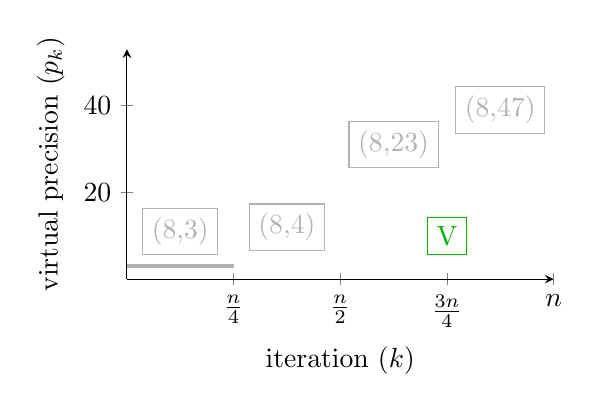
\begin{tikzpicture}
\begin{axis}[width=7cm,
            height=4.5cm,
            axis y line=center,
            axis x line=middle,
            xmax=4, 
            ymin=0,
            ymax=53,
            xlabel=iteration ($k$), 
            ylabel=virtual precision ($p_k$), 
            ylabel near ticks, 
            xlabel near ticks,
            xticklabels={0,0,$\frac{n}{4}$,$\frac{n}{2}$,$\frac{3n}{4}$,$n$},
]
\only<14>{
\addplot[mark=none, black, ultra thick, opacity=.3] coordinates {(0,3) (1,3)};
\node[draw, opacity=.3] at (axis cs:.5,11) {(8,3)};
\addplot[mark=none, black, ultra thick, opacity=.] coordinates {(1,4) (2,4)};
\node[draw, opacity=.3] at (axis cs:1.5,12) {(8,4)};
\addplot[mark=none, black, ultra thick, opacity=.] coordinates {(2,23) (3,23)};
\node[draw, opacity=.3] at (axis cs:2.5,31) {(8,23)};
\addplot[mark=none, black, ultra thick, opacity=.] coordinates {(3,47) (4,47)};
\node[draw, opacity=.3] at (axis cs:3.5,39) {(8,47)};
\node[draw, black!30!green] at (axis cs:3,10) {V};
}

\end{axis}
\end{tikzpicture}

}


\only<15>{

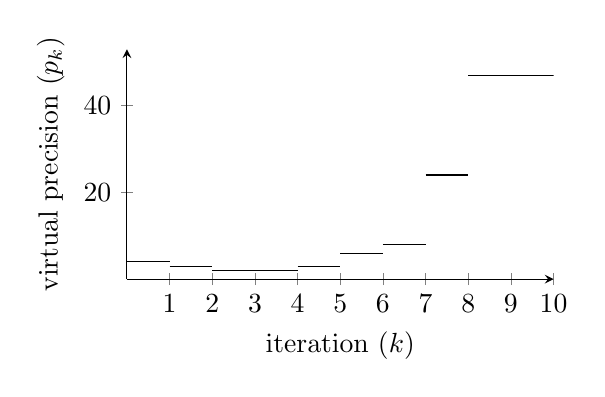
\begin{tikzpicture}
\begin{axis}[width=7cm,
            height=4.5cm,
            axis y line=center,
            axis x line=middle,
            xmax=10, 
            ymin=0,
            ymax=53,
            xlabel=iteration ($k$), 
            ylabel=virtual precision ($p_k$), 
            ylabel near ticks, 
            xlabel near ticks,
            xtick={0,1,2,3,4,5,6,7,8,9,10},
            xticklabels={0,1,2,3,4,5,6,7,8,9,10},
]
\only<15>{
\addplot[mark=none, black] coordinates {(0,4) (1,4)};
\addplot[mark=none, black] coordinates {(1,3) (2,3)};
\addplot[mark=none, black] coordinates {(2,2) (3,2)};
\addplot[mark=none, black] coordinates {(3,2) (4,2)};
\addplot[mark=none, black] coordinates {(4,3) (5,3)};
\addplot[mark=none, black] coordinates {(5,6) (6,6)};
\addplot[mark=none, black] coordinates {(6,8) (7,8)};
\addplot[mark=none, black] coordinates {(7,24) (8,24)};
\addplot[mark=none, black] coordinates {(8,47) (9,47)};
\addplot[mark=none, black] coordinates {(9,47) (10,47)};
}

\end{axis}
\end{tikzpicture}

}

\end{figure}

\end{frame}

%\begin{frame}{Exploration step-by-step}
%\begin{figure}
%    \centering
%    \only<1>{\includegraphics[width=\linewidth]{images/gif/0.jpg}}
\only<2>{\includegraphics[width=\linewidth]{images/gif/1.jpg}}
\only<3>{\includegraphics[width=\linewidth]{images/gif/2.jpg}}
\only<4>{\includegraphics[width=\linewidth]{images/gif/3.jpg}}
\only<5>{\includegraphics[width=\linewidth]{images/gif/4.jpg}}
\only<6>{\includegraphics[width=\linewidth]{images/gif/5.jpg}}
\only<7>{\includegraphics[width=\linewidth]{images/gif/6.jpg}}
\only<8>{\includegraphics[width=\linewidth]{images/gif/7.jpg}}
\only<9>{\includegraphics[width=\linewidth]{images/gif/8.jpg}}
\only<10>{\includegraphics[width=\linewidth]{images/gif/9.jpg}}
\only<11>{\includegraphics[width=\linewidth]{images/gif/10.jpg}}
\only<12>{\includegraphics[width=\linewidth]{images/gif/11.jpg}}
\only<13>{\includegraphics[width=\linewidth]{images/gif/12.jpg}}
\only<14>{\includegraphics[width=\linewidth]{images/gif/13.jpg}}
\only<15>{\includegraphics[width=\linewidth]{images/gif/14.jpg}}
\only<16>{\includegraphics[width=\linewidth]{images/gif/15.jpg}}
\only<17>{\includegraphics[width=\linewidth]{images/gif/16.jpg}}
\only<18>{\includegraphics[width=\linewidth]{images/gif/17.jpg}}
\only<19>{\includegraphics[width=\linewidth]{images/gif/18.jpg}}
\only<20>{\includegraphics[width=\linewidth]{images/gif/19.jpg}}
\only<21>{\includegraphics[width=\linewidth]{images/gif/20.jpg}}
\only<22>{\includegraphics[width=\linewidth]{images/gif/21.jpg}}
\only<23>{\includegraphics[width=\linewidth]{images/gif/22.jpg}}
\only<24>{\includegraphics[width=\linewidth]{images/gif/23.jpg}}
\only<25>{\includegraphics[width=\linewidth]{images/gif/24.jpg}}
\only<26>{\includegraphics[width=\linewidth]{images/gif/25.jpg}}
\only<27>{\includegraphics[width=\linewidth]{images/gif/26.jpg}}
\only<28>{\includegraphics[width=\linewidth]{images/gif/27.jpg}}
\only<29>{\includegraphics[width=\linewidth]{images/gif/28.jpg}}
\only<30>{\includegraphics[width=\linewidth]{images/gif/29.jpg}}
\only<31>{\includegraphics[width=\linewidth]{images/gif/30.jpg}}
\only<32>{\includegraphics[width=\linewidth]{images/gif/31.jpg}}
\only<33>{\includegraphics[width=\linewidth]{images/gif/32.jpg}}
\only<34>{\includegraphics[width=\linewidth]{images/gif/33.jpg}}
\only<35>{\includegraphics[width=\linewidth]{images/gif/34.jpg}}
\only<36>{\includegraphics[width=\linewidth]{images/gif/35.jpg}}
\only<37>{\includegraphics[width=\linewidth]{images/gif/36.jpg}}
\only<38>{\includegraphics[width=\linewidth]{images/gif/37.jpg}}
\only<39>{\includegraphics[width=\linewidth]{images/gif/38.jpg}}
\only<40>{\includegraphics[width=\linewidth]{images/gif/39.jpg}}
\only<41>{\includegraphics[width=\linewidth]{images/gif/40.jpg}}
\only<42>{\includegraphics[width=\linewidth]{images/gif/41.jpg}}
\only<43>{\includegraphics[width=\linewidth]{images/gif/42.jpg}}
\only<44>{\includegraphics[width=\linewidth]{images/gif/43.jpg}}
\only<45>{\includegraphics[width=\linewidth]{images/gif/44.jpg}}
\only<46>{\includegraphics[width=\linewidth]{images/gif/45.jpg}}
\only<47>{\includegraphics[width=\linewidth]{images/gif/46.jpg}}
\only<48>{\includegraphics[width=\linewidth]{images/gif/47.jpg}}
\only<49>{\includegraphics[width=\linewidth]{images/gif/48.jpg}}
\only<50>{\includegraphics[width=\linewidth]{images/gif/49.jpg}}
\only<51>{\includegraphics[width=\linewidth]{images/gif/50.jpg}}
\only<52>{\includegraphics[width=\linewidth]{images/gif/51.jpg}}
\only<53>{\includegraphics[width=\linewidth]{images/gif/52.jpg}}
\only<54>{\includegraphics[width=\linewidth]{images/gif/53.jpg}}
\only<55>{\includegraphics[width=\linewidth]{images/gif/54.jpg}}
\only<56>{\includegraphics[width=\linewidth]{images/gif/55.jpg}}
\only<57>{\includegraphics[width=\linewidth]{images/gif/56.jpg}}
\only<58>{\includegraphics[width=\linewidth]{images/gif/57.jpg}}
\only<59>{\includegraphics[width=\linewidth]{images/gif/58.jpg}}
\only<60>{\includegraphics[width=\linewidth]{images/gif/59.jpg}}
\only<61>{\includegraphics[width=\linewidth]{images/gif/60.jpg}}
\only<62>{\includegraphics[width=\linewidth]{images/gif/61.jpg}}
\only<63>{\includegraphics[width=\linewidth]{images/gif/62.jpg}}
\only<64>{\includegraphics[width=\linewidth]{images/gif/63.jpg}}
\only<65>{\includegraphics[width=\linewidth]{images/gif/64.jpg}}
\only<66>{\includegraphics[width=\linewidth]{images/gif/65.jpg}}
\only<67>{\includegraphics[width=\linewidth]{images/gif/66.jpg}}
\only<68>{\includegraphics[width=\linewidth]{images/gif/67.jpg}}
\only<69>{\includegraphics[width=\linewidth]{images/gif/68.jpg}}
\only<70>{\includegraphics[width=\linewidth]{images/gif/69.jpg}}
\only<71>{\includegraphics[width=\linewidth]{images/gif/70.jpg}}
\only<72>{\includegraphics[width=\linewidth]{images/gif/71.jpg}}
\only<73>{\includegraphics[width=\linewidth]{images/gif/72.jpg}}
\only<74>{\includegraphics[width=\linewidth]{images/gif/73.jpg}}
\only<75>{\includegraphics[width=\linewidth]{images/gif/74.jpg}}
\only<76>{\includegraphics[width=\linewidth]{images/gif/75.jpg}}
\only<77>{\includegraphics[width=\linewidth]{images/gif/76.jpg}}
\only<78>{\includegraphics[width=\linewidth]{images/gif/77.jpg}}
\only<79>{\includegraphics[width=\linewidth]{images/gif/78.jpg}}
\only<80>{\includegraphics[width=\linewidth]{images/gif/79.jpg}}
\only<81>{\includegraphics[width=\linewidth]{images/gif/80.jpg}}
\only<82>{\includegraphics[width=\linewidth]{images/gif/81.jpg}}
\only<83>{\includegraphics[width=\linewidth]{images/gif/82.jpg}}
\only<84>{\includegraphics[width=\linewidth]{images/gif/83.jpg}}
\only<85>{\includegraphics[width=\linewidth]{images/gif/84.jpg}}
\only<86>{\includegraphics[width=\linewidth]{images/gif/85.jpg}}
\only<87>{\includegraphics[width=\linewidth]{images/gif/86.jpg}}
\only<88>{\includegraphics[width=\linewidth]{images/gif/87.jpg}}
%    \caption{Piecewise constant exploration on Newton-Raphson.}
%    \label{fig:my_label}
%\end{figure}
%\end{frame}

\begin{frame}{Exploration on an industrial use case: YALES2}

\begin{figure}
    \centering
    
\includegraphics[width=0.5\linewidth,keepaspectratio]{Logo_YALES2.jpg}
    \caption*{Coria-CNRS and Safran, Solvay, GDF-Suez, \href{https://www.coria-cfd.fr}{www.coria-cfd.fr}}
\end{figure}

\begin{block}{\textbf{\alert{Solver for two-phase combustion}}}
\begin{itemize}
    \item From primary atomization to pollutant prediction
\end{itemize}
\end{block}

\begin{block}{\textbf{\alert{Deflated Preconditioned Conjugate Gradient}}}
\begin{itemize}
    \item A fine grid is geometrically projected on a coarse grid
    \item A CG is applied on the coarse grid and on the fine grid
\end{itemize}
\end{block}

\begin{block}{\textbf{\alert{\emph{Preccinsta burner} use case}}}
\begin{itemize}
    \item Evaluation on 1.75 million mesh elements
%    \item Scaling from 1 to 560 cores on CRIANN cluster (66 bisocket Intel Xeon E5-2680 nodes and Intel Omnipath interconnect)
    \item Exploring reduction on \alert{\emph{entire application}} and \alert{\emph{deflated grid}} 
\end{itemize}
\end{block}
\end{frame}

\begin{frame}[fragile]{Deflated Preconditioned Conjugate Gradient}
  \vspace{-2mm}
\begin{block}{A-DEF2 using preconditioner $M^{-1}$ and deflation matrix $W$.}
    \begin{itemize}
        \item In blue the \colorbox{blue!25}{coarse grid} and green the \colorbox{green!20}{fine grid}
        \item \alert{deflated part} = \colorbox{blue!25}{blue}, \alert{entire application} = \colorbox{green!20}{green} + \colorbox{blue!25}{blue}
    \end{itemize}
\end{block}
\vspace{-5mm}
\begin{figure}
  \begin{lstlisting}[escapeinside={(*}{*)}, mathescape=true, basicstyle=\small, captionpos=b ]
(* \textbf{Require} *): $A,b,M^{-1},W$
(* \textbf{initialization} *)
(* \textbf{for} *) k = 0,1,... until required convergence (* \textbf{do} *)
    (* \colorbox{green!20}{$\alpha_{k+1} = \dfrac{ r^T_k w_k }{ p^T_k A p_k}$    }     *)
    (* \colorbox{green!20}{$ x_{k+1} = x_k + \alpha_{k+1} p_k $                  }                   *)
    (* \colorbox{green!20}{$ r_{k+1} = r_k - \alpha_{k+1} A p_k $                }                 *)
    (* \colorbox{blue!25}{Solve $\hat{A}d_{k+1} = W^{T}(AM^{-1}-I)r_{k+1} $      }       *)
    (* \colorbox{green!20}{$ w_{k+1} = M^{-1} r_{k+1} - W d_{k+1} $              }               *)
    (* \colorbox{green!20}{$ \beta_{k+1} = \dfrac{ r^T_k w_{k+1} }{ r^T_k w_k } $} *)
    (* \colorbox{green!20}{$ p_{k+1} = w_{k+1} + \beta_{k+1} p_k $               }                *)
(* \textbf{end for} *)
\end{lstlisting}
\end{figure}

\end{frame}


\begin{frame}{Piecewise constant exploration on \emph{preccinsta 1.75M}}
    
\begin{figure}
    \centering
    \begin{tabular}{cl}
    \multicolumn{2}{c}{
\includegraphics[width=\linewidth]{images/legend-4.pdf}} \\
    Entire application & Deflated part \\
    
\includegraphics[width=.49\linewidth]{images/upper-left.pdf} & 
\includegraphics[width=.49\linewidth]{images/upper-right.pdf} \\
    
\includegraphics[width=.49\linewidth]{images/bottom-left.pdf} & 
\includegraphics[width=.49\linewidth]{images/bottom-right.pdf} \\
    \end{tabular}
    \vspace{-6mm}
    \caption{Adaptive precision searching on YALES2's DPCG on 1 MPI. 
    $\mathbf{r=8}$.
    Reduced precision solution follows the reference IEEE convergence profile}
    \label{fig:deflated_piecewise_GC}
\end{figure}

\end{frame}

\begin{frame}{Validating resiliency to round-off errors}
\begin{block}{\alert{VPREC is a deterministic computation model}}
\begin{itemize}
    \item How to validate configuration's robustness to rounding errors?
\end{itemize}
\end{block}
\vspace{-2mm}
\begin{block}{\alert{Using Monte Carlo Arithmetic~\cite{parker1997monte}}}
    \vspace{-2mm}
    \begin{itemize}
        \item Introduces random noise to \alert{model round-off errors} at 
        each FP ops
        \item Used as \alert{second step} for validating VPREC configurations
        \item 29 converged MCA samples gives 90\% of probability with 0.95 confidence level based on Bernouilli trials~\cite{sohier} that configuration is robust to round-off errors
    \end{itemize}
\end{block}
\vspace{-2mm}
\begin{figure}
    \centering
    \begin{minipage}{0.49\linewidth}
    
\includegraphics[width=\linewidth]{right-envelop-vprec.pdf}
    \end{minipage}
    \begin{minipage}{0.49\linewidth}
    
\includegraphics[width=0.75\linewidth]{legend-3.pdf}
    \end{minipage}
\end{figure}
\end{frame}

\begin{frame}{Performance validation on mixed-precision version}
    \begin{itemize}
        \item \alert{Mixed-version} to use both \texttt{binary32} and \texttt{binary64} formats in the deflated operator
        \item Switch from \texttt{binary32} to \texttt{binary64} when
        convergence criteria is below $10^{-7}$
        \item Run up to 560 cores on CRIANN cluster (66 bisocket Intel Xeon E5-2680 nodes and Intel Omnipath interconnect)
    \end{itemize}
    \begin{figure}
    \begin{minipage}{0.49\linewidth}
    
\includegraphics[width=\linewidth]{gains_comm.pdf}    
    \end{minipage}    
    \begin{minipage}{0.49\linewidth}
    
\includegraphics[width=\linewidth]{gains_speedup.pdf}
    \end{minipage}
    \end{figure}
\end{frame}

\begin{frame}{Conclusion}
    \begin{block}{\textbf{\alert{VPREC}}}
    \begin{itemize}
        \item Easily tests \alert{custom formats} on HPC codes
    \end{itemize}
    \end{block}
    \begin{block}{\textbf{\alert{Find lowest precision}}}
    \begin{itemize}
        \item \alert{Automatic search} to find lowest precision 
        \item Reduces working precision while preserving \alert{accuracy} and \alert{convergence}
        \item \alert{Robustness} to rounding errors thanks to MCA
    \end{itemize}
    \end{block}
    \begin{block}{\textbf{\alert{Validation on industrial code Yales2}}}
    \begin{itemize}
        \item Mixed-precision version \alert{scaling} up to 560 cores
        \item Average \alert{communications' volume} reduction by \alert{\textbf{30\%}}
        and \alert{best speedup} of \alert{\textbf{1.28}}
    \end{itemize}
    \end{block}
\end{frame}

\appendix

\begin{frame}{Backup slides}
    
\end{frame}

\begin{frame}{IEEE-754 formats}
\begin{table}[]
    \centering
    \begin{tabular}{l|c|c|c}
        Name & Exponent & Pseudo-Mantissa & $e_{min},e_{max}$ \\
             & (bits)          & (bits) & \\
        \hline
        \hypertarget{binaryH}{binary16} & 5 & 10 & (-14,+15) \\ 
        \hypertarget{binaryS}{binary32} & 8 & 23 & (-126,+127) \\
        \hypertarget{binaryD}{binary64} & 11 & 52 & (-1022,+1023) \\
        \hypertarget{binaryQ}{binary128} & 15 & 112 & (-16382,+16383) \\
    \end{tabular}
    \caption{Binary formats of the IEEE-754 norme}
    \label{tab:formats-binaires-ieee}
\end{table}
\end{frame}

\begin{frame}{Accelerate the convergence}
\begin{figure}
    \centering
    
\includegraphics[width=\linewidth]{precinsta_850M_112.png}
    \caption*{Exploration on \emph{preccinsta} 850M on 112 MPI cores on
    deflated part.
    Solution found by the exploration (\emph{VPREC}) converges in 66 iterations
    while the original (\emph{Double}) converges in 100 iterations. \\
    Reducing precision can be seen as a high-pass filter. \\
    75\% of solutions found by VPREC used less iterations than the IEEE version
    }
\end{figure}
\end{frame}

\begin{frame}{Billion mesh elements}
    \begin{figure}
        
\includegraphics[width=\linewidth]{big_336_preccinsta_Y2.pdf}
        \caption*{Exploration on \emph{preccinsta} with billion of elements on 336 MPI cores. VPREC exploration shows that we need more precision 
        at the end to reach the convergence. Fix $r=8$}
    \end{figure}
\end{frame}

\begin{frame}[allowframebreaks]{References}

  \bibliography{main}
  \bibliographystyle{apalike}

\end{frame}

\end{document}
